\section{Discussion}

This section synthesises the experimental findings and discusses their implications for practical watermark verification in diffusion-based generative models, with particular emphasis on robustness, generalisation, and deployment-oriented evaluation.

\subsection{Overall Robustness of the Learned Detector}

The results consistently demonstrate that SpiderMark achieves strong and stable watermark verification across a wide range of photometric, geometric, and mixed distortions. Unlike handcrafted similarity metrics, the learned verifier maintains reliable performance even under aggressive transformations such as strong JPEG compression, spatial resampling, and partial occlusion.

Importantly, the detector’s robustness extends beyond pixel-level fidelity. The sustained performance under spatial misalignment and local corruption suggests that the watermark signal is encoded in structured frequency-domain patterns that propagate through the diffusion process and remain detectable after substantial post-processing. This confirms that the proposed injection strategy produces a watermark that is both imperceptible and structurally persistent, while the learned verifier effectively captures these stable cues.

\subsection{Limitations of AUC as a Robustness Metric}\label{subsec:auc_limitations}


\begin{figure*}
    \centering
    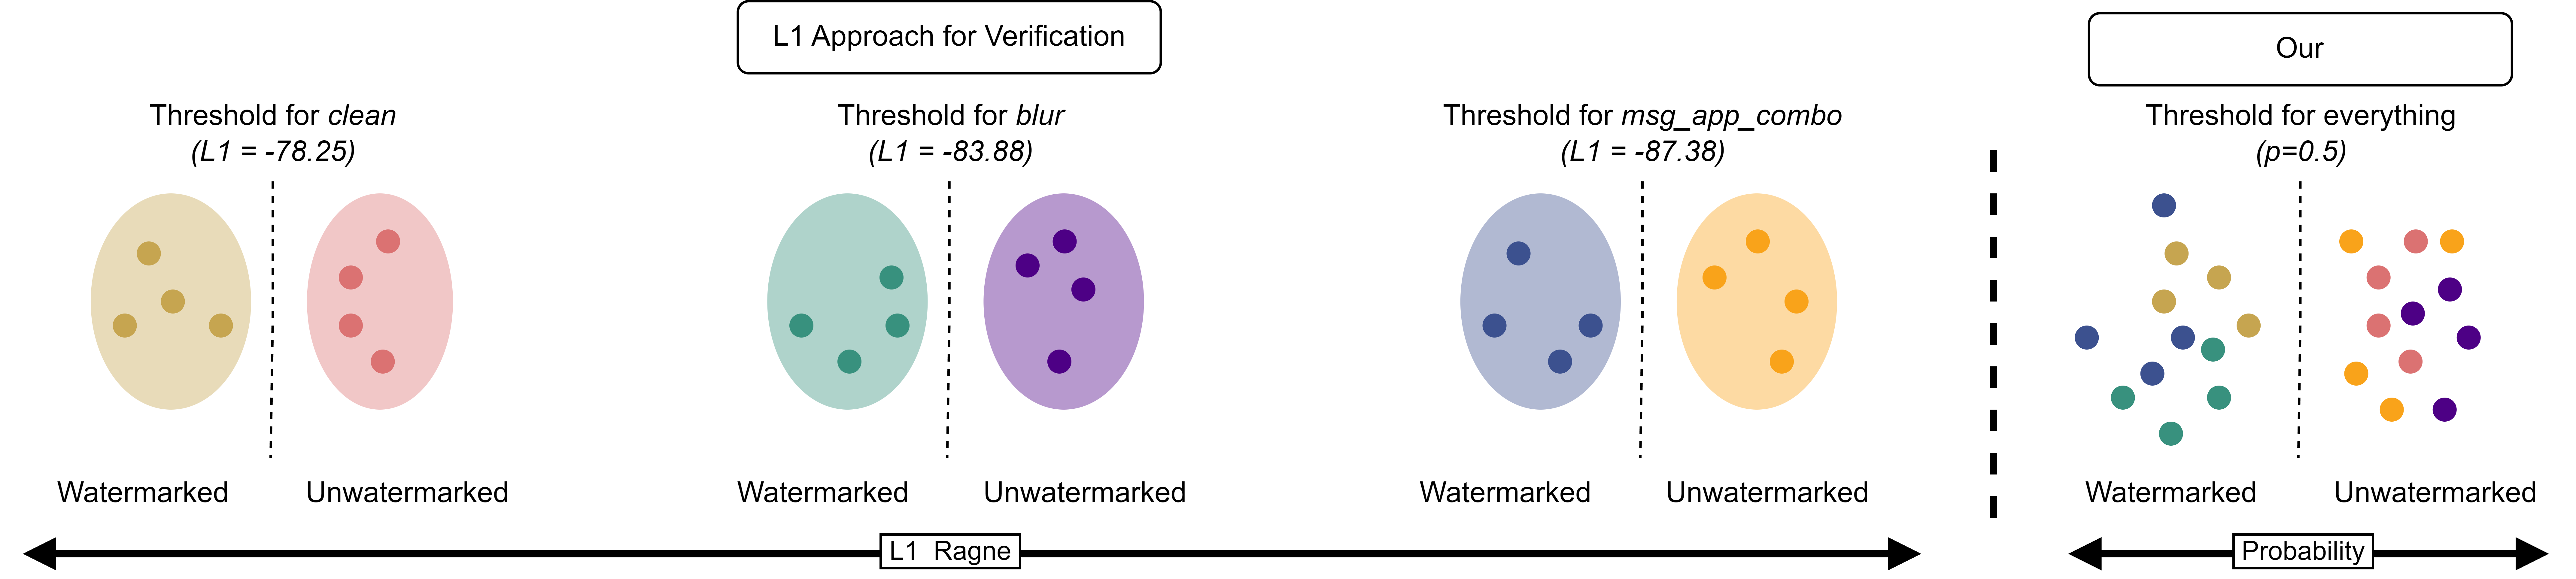
\includegraphics[width=1\linewidth]{figures/l1_not_best.png}
    \caption{Conceptual comparison between L1-distance--based verification and our probabilistic verification approach. 
        \textbf{Left:} Under different attacks, the distributions of L1 distances for watermarked and unwatermarked images shift in an attack-dependent manner, resulting in no single universal decision threshold.
        \textbf{Right:} Our method maps verification evidence to calibrated probabilities, enabling more stable and attack-invariant decision-making without relying on a fixed distance threshold.}
    \label{fig:l1_limitations}
\end{figure*}



Although AUROC is a common metric for evaluating binary classifiers, our experiments highlight its limitations for assessing watermark robustness in real-world deployment scenarios. In practice, watermark verification systems must operate at a \emph{fixed decision threshold}, whereas AUROC evaluates separability by sweeping over all possible thresholds. As a result, a high AUROC does not necessarily translate into reliable verification performance at inference time.

As shown in Table~\ref{tab:threshold_shift}, the optimal thresholds for distance-based detectors such as L1 or PSNR vary substantially across different attack types. This threshold instability persists even when AUROC remains high, indicating that separability alone is insufficient to guarantee robustness under unknown or mixed distortions.

Figure~\ref{fig:l1_limitations} provides an intuitive illustration of this phenomenon. Scalar distance metrics induce attack-dependent shifts in score distributions, making it impossible to select a single universal threshold. In contrast, the proposed verifier maps frequency-domain evidence to calibrated probabilities, enabling more stable decision-making under a fixed operating point. This probabilistic formulation is therefore better aligned with real-world deployment constraints.

\subsection{Photometric Robustness}

Under photometric degradations such as strong JPEG compression and Gaussian blur, SpiderMark substantially outperforms PSNR-based verification, which collapses to near-random performance. The resilience of the learned detector indicates that it leverages mid-frequency spectral structures that survive quantisation and smoothing, rather than relying on fragile pixel-level statistics.

This robustness is particularly important in real-world content distribution pipelines, where images are routinely re-encoded, resized, or compressed by platforms beyond the control of the content creator or verifier.

\subsection{Geometric and Spatial Robustness}

Spatial transformations such as downsampling–upsampling, geometric warping, and random cropping pose significant challenges for watermark verification due to spatial misalignment. Despite these distortions, SpiderMark maintains strong AUROC and accuracy, demonstrating that the verifier learns geometry-invariant watermark signatures in the frequency domain.

In contrast, classical baselines that depend on pixel alignment or fixed spatial correspondence degrade sharply once spatial consistency is disrupted. These results highlight the advantage of combining noise-level frequency injection with learned verification over rigid, handcrafted detection rules.

\subsection{Effect of Watermark Pattern and Mask (PM) Ablation}

The ablation study reveals that providing the watermark pattern and mask as auxiliary inputs generally improves verification robustness, particularly under compression, occlusion, and resampling. These components act as structural priors, guiding the verifier toward watermark-relevant spectral regions.

However, under severe geometric distortions such as random cropping, the spatial alignment between the pattern and the observed image may be compromised, reducing the benefit of explicit pattern conditioning. In such cases, the PM-agnostic model performs comparably, suggesting that augmentation-aware training could further enhance robustness when strong spatial perturbations are expected.

\subsection{Cross-Dataset Generalisation}

A key finding of this work is the strong generalisation of the verifier to unseen data distributions. Although the verifier is trained exclusively on images generated from the Stable Diffusion prompt dataset, it consistently achieves the best performance on the COCO dataset without any retraining or fine-tuning.

This result indicates that the verifier does not overfit to prompt-specific semantics or dataset-specific artefacts, but instead learns watermark-consistent frequency-domain cues that transfer across datasets. Such generalisation is essential for practical deployment, where the verifier may encounter images generated under diverse prompts, styles, or downstream usage contexts.

\subsection{Semantic Preservation and Perceptual Quality}

The CLIP-based semantic evaluation further confirms that SpiderMark introduces negligible semantic distortion. The observed differences in CLIP similarity between watermarked and unwatermarked images are consistently below 0.003 across both Stable Diffusion and COCO datasets, which is well below commonly accepted thresholds for perceptual or semantic degradation.

In conjunction with comparable FID scores, these results demonstrate that improved robustness does not come at the expense of image quality or semantic fidelity, reinforcing the practicality of the proposed approach.

\subsection{Implications for Real-World Deployment}

Taken together, these findings establish SpiderMark as a practical and deployment-ready watermarking framework for diffusion-based generative models. By combining noise-level frequency injection with probabilistic, threshold-aware verification, the proposed system addresses key limitations of existing watermarking approaches, including threshold instability, poor robustness under transformation, and limited generalisation.

The analysis also highlights the importance of evaluation protocols that reflect real-world operating constraints. Metrics that account for fixed thresholds and calibrated confidence scores provide a more faithful assessment of robustness than threshold-free measures such as AUROC alone. These insights are broadly applicable beyond watermarking and may inform the evaluation of other content attribution and authenticity systems.
